\documentclass[a4paper,11pt,onecolumn]{article}
\usepackage[hscale=0.8,vscale=0.9]{geometry}
\usepackage[parfill]{parskip}
\usepackage{amsmath}
\usepackage{amsfonts}
\usepackage{graphicx}
\usepackage{subfigure}
\usepackage{wrapfig}
\usepackage{amssymb}

\newcommand{\eat}[1]{}

\begin{document}
\include{weld-defns}
\title{Research Statement}
\author{Niranjan Balasubramanian}
\maketitle

My research spans two broad areas: Information retrieval and Natural Language Processing. Applications such as web search, information extraction, summarization and question answering provide easy access to the vast amounts information on the web. These challenging applications require computer systems to extract, understand and reason with knowledge present in natural language texts. This long-standing Artificial Intelligence (AI) vision has tremendous societal and scientific impacts. My research is motivated by this vision and aims at building large scale open domain knowledge targeted towards specific applications.

Consider a system answering a 4th grade science question:  ``Which is the best conductor of electricity? (A) metal fork (B) rubber boat''. The system needs access to the knowledge that i) a metal fork is made of metal, ii) metals conduct electricity, and iii) properties of a metal apply to things made of metal. It also needs to reason with this knowledge to arrive at the answer. Consider an event extraction system that is ``reading" an article about an arrest event. If the system had knowledge about what a typical arrest event is -- i.e., who the key actors are and what their roles are -- then it can use that information to identify the salient pieces to extract from the article. 

My current research focuses on developing methods for extracting such large scale open-domain knowledge and robust mechanisms for applying this knowledge. For wide applicability, I target methods that meet the following design goals: Scale to arbitrary domains, model semantics without ambiguity, and generalize to unseen contexts. %I use scalable Open Information Extraction (Open IE) techniques to extract open-domain relations fashion and build representations with semantic classes to reduce ambiguity and improve generalization.

%My research methods are centered on identifying the core aspects of the problem space through careful analysis of existing systems and data. For instance, in my work on event schemas, I analyzed output from a previous system and identified the key shortcomings of underspecified representations. The insights led to a better representation that vastly improved the quality of the schemas. In my work on mobile search, I conducted a systematic study of data transfer costs in cellular networks. This study identified a key energy inefficiency, which spawned a large body of research aimed at minimizing its impact.~\footnote{This work has more than 350 citations.} 

Here I describe some of my research and lay out my vision for future work.

\subsection*{NLP [EMNLP 2013, AKBC-WEKEX 2012, 2013]}

{\bf Modeling Events}

Event schemas specify actors and their roles within events. 
They are widely used in event extraction. 
Figure~\ref{fig:arrest} shows an example arrest schema. 
The key actors are an arresting agent who arrests and charges a suspect, a lawyer who represents the suspect and a judge who rules on the case. 
\begin{wrapfigure}{lh}{0.4\textwidth}
	\vspace{-2ex}
	\begin{center}
	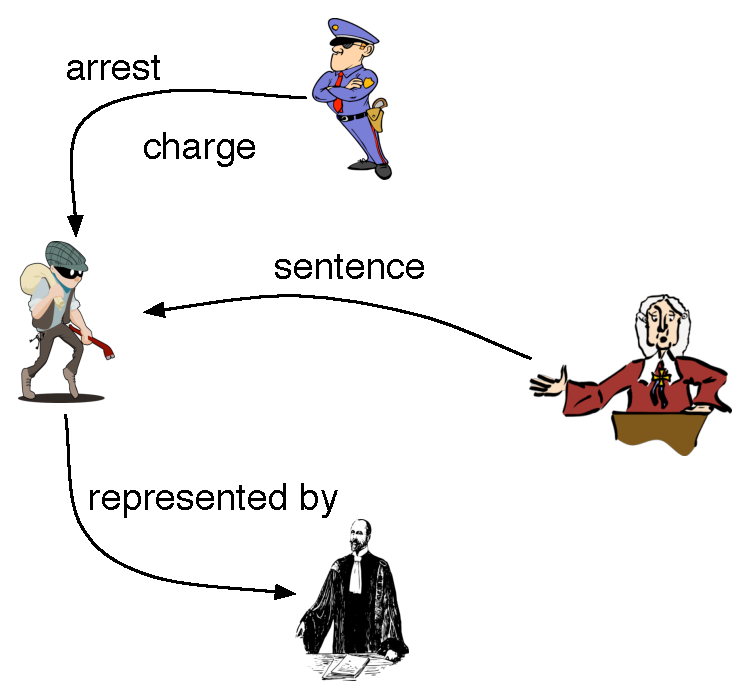
\includegraphics[width=2.5in,height=2in]{figures/arrest-scenario} 	
	\vspace{-2ex}
	\caption{\label{fig:arrest} {\small Arrest schema: A model for an arrest scenario including key actors, the police, the suspect, judge etc. and their roles.}}
	\vspace{-4ex}
	\end{center}
\end{wrapfigure}
My research aims to automatically generate these schemas from text without any manual effort. 

The main premise behind my work is that an accurate model of co-occurring actors and their actions can provide a basis for automatically generating schemas. The main challenge is in defining a suitable representation for the actions. My analysis of the output from a previous system showed that simpler (subject, verb) and (verb, object) pairs are underspecified and split critical context. In response, I developed an Open IE triple-based solution that uses a (Arg1, Relation, Arg2) triple that captures more specific information about the actions and reduces ambiguity. However, this reduction in ambiguity comes at a cost of increased sparsity and reduced generalization. 
To counter this issue, I represent arguments using semantic classes, which allows the model to generalize beyond the specific entities to new unseen contexts. The relational co-occurrence model (Rel-grams) built over this triple representation yields a form of entailment type knowledge~\cite{balasubramanian-akbc12} and produces schemas that are more coherent than state-of-the-art systems~\cite{balasubramanian-emnlp13}.


{\bf Question Answering}

Achieving human-level performance on tasks that require intelligence has a long tradition in the history of AI. As one of the foundational members of the Allen Institute for Artificial Intelligence, I am co-leading efforts to design and develop a QA system that is capable of passing a 4th grade science exam.~\footnote{I also contribute to the long term research planning and have written grant proposals with Dr. Oren Etzioni that secured funding on earlier versions of this project.} This is an exciting long-term research project that seeks to address several fundamental challenges in representation, extraction, and reasoning all in the context of a single task. 
\begin{wrapfigure}{lh}{0.6\textwidth}
	\begin{center}
	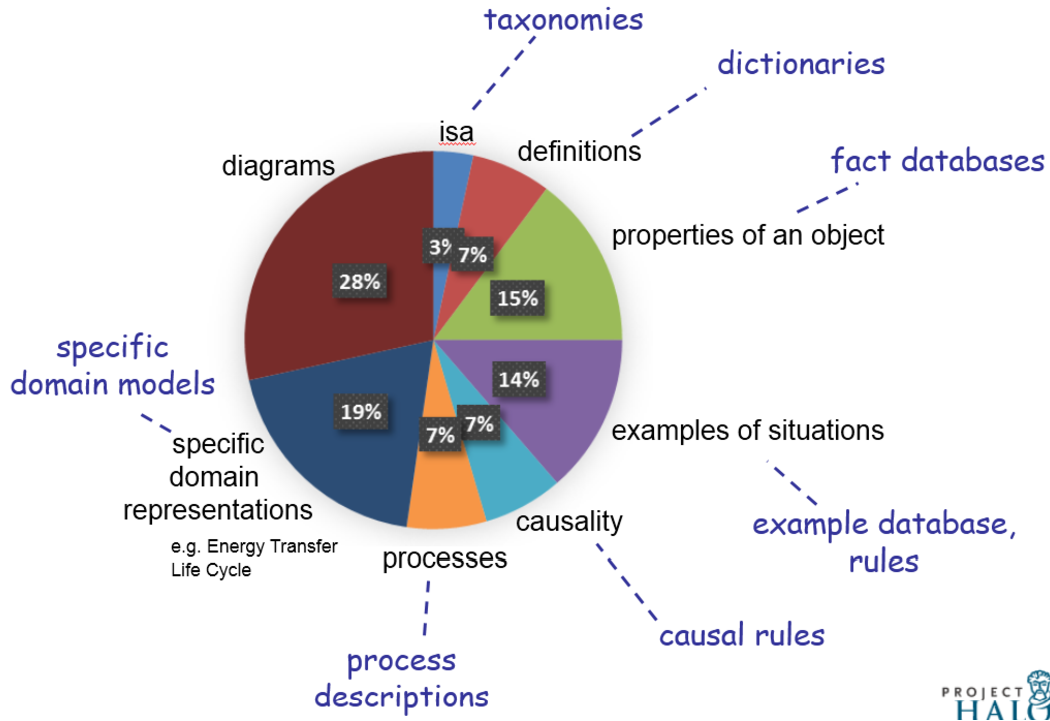
\includegraphics[width=3in,height=2in]{figures/akbc} 	
	\vspace{-2ex}
	\caption{\label{fig:akbc} {\small Knowledge Requirements for a 4th Grade Science Exam}}
	\vspace{-2ex}
	\end{center}
\end{wrapfigure}

As a first step, we studied the knowledge requirements for passing a 4th grade science exam~\cite{clark-akbc13}. The knowledge requirements summarized in Figure~\ref{fig:akbc} shows that this is a challenging task requiring a wide range of knowledge and robust reasoning methods. In addition to factual knowledge (e.g., iron conducts electricity), we identify three other types of useful knowledge: 1) Definitional knowledge, 2) Domain knowledge expressed via general purpose relations such as cause/effect, entity/function, 3) Implications representing domain and background knowledge (e.g., animal breathes oxygen $-$enables$\rightarrow$ animal make energy), and 4) Qualitative domain models (e.g., Reasoning with predator-prey models: If population of snakes rise, what happens to the population of frogs?).

We are building a wide array of solutions to address these difficult challenges. We extract definitional and general purpose relations such as cause/effect and entity/function using hand-generated lexico-syntactic patterns that exploit strong regularities in language. We use Open IE style relations to represent information but expand them to cover nested relations. In addition, we also use facts extracted using a state-of-the-art Open IE extractor. Our preliminary experiments show about 15\% improvement over simple keyword search baselines.

\subsection*{Information Retrieval [SIGIR 2010, CIKM 2009, IMC 2009, CoNext 2012]}

{\bf Combining Alternatives}

The IR research community continuously develops query representations, retrieval models, and various ranking algorithms. As part of my thesis, I developed a dynamic query-dependent approach for combining different alternatives. The main premise behind my thesis is that different alternatives work well for different queries. For example, a navigation query (intent to visit a specific url) is well served by click-based features, whereas a informational query is better served by query-document match features. If we can select the best choice(s) for a given query, then we can further improve retrieval performance. 

To this end, I developed a novel method that estimates the relative performance of the alternatives with respect to a baseline~\cite{balasubramanian-sigir10a}. The key insight behind this method was that accurate estimation of the absolute effectiveness value was not essential. The estimation only needed to induce a good ordering of the available alternatives. This relative estimation method outperformed using the single best alternative for query representations~\cite{balasubramanian-sigir10b} and standard fusion methods for combining ranking functions~\cite{balasubramanian-sigir10c}. 


{\bf Topic Pages}

As an alternative to the typical web search paradigm, I built a system that automatically generates wikipedia like pages for queries~\cite{balasubramanian-icsc2010}. The primary challenge here is to identify the salient but diverse aspects pertaining to the query topic. I used web search logs to build diverse aspect models on topics. To generalize to topics beyond those that are observed in the search logs, I generalized the aspect models to include information from related topics. A second challenge here is to extract and organize information pertaining to the diverse aspects in a coherent fashion. I built a sentence extractor that identifies most typical connection between the topic and its aspect and used simple word-precedence models to organize the retrieved sentences. The resulting topic pages outperformed state-of-the-art summarization systems in terms of grammaticality, salience and coherence.

{\bf Mobile Search}

I studied the impact of system constraints on web search from mobile phones. I conducted a systematic study of how network activity consumed energy in mobile phones. My study revealed that energy consumption also depended on inter-transfer times in addition to the size of the data being transferred~\cite{balasubramanian-imc09}. Based on this insight, I designed interaction strategies that reduced the energy consumption of web search applications. In addition to improving the energy efficiency of web search, the key finding in this work led to a large body of work aimed at addressing the energy inefficiency.

I also worked on {\em FindAll}, a mobile search engine aimed at improving local availability of previously visited documents. Because indexing on the phone is expensive, the system must balance local availability against resource usage and energy consumption. Using actual search logs from mobile users, we learned user-specific re-finding patterns to predict when a user is likely to re-find documents. Using this predictive model, FindAll selectively indexes documents when cost of indexing is lower than cost of re-finding the document over the network. Evaluations show that FindAll dramatically improves local availability for heavy users without increasing the energy costs.

\subsection*{Future Work}

Building systems that can understand and reason with natural language texts is one of the central visions of AI. 	 
I am interested in three veins of research that build towards this vision: 
\begin{enumerate}
\item Acquiring richer knowledge forms -- Extracting and understanding information in texts itself requires background knowledge. For example models of salient aspects of certain types of entities (e.g., actors play movies, win awards) can help extract and organize information about people. Similarly, rich descriptions of events or scenarios, processes and their interactions can help in extracting and understanding information about events from texts. Scalable methods for acquiring such background knowledge is essential for extracting richer structures from text.  
\item Reasoning with knowledge from texts -- Much of world's knowledge is already available in the form of natural language texts. While extraction capabilities are improving, they have several issues that need to be addressed in order to be useful for end applications. 
\item Semantic search capabilities -- Advent of scalable extraction and language processing capabilities present a great opportunity to push information retrieval toward more semantic representations and retrieval models.
\end{enumerate}
%i) Acquiring richer knowledge to aid extraction, ii) Reasoning with automatically extracted knowledge, and iii) Using semantic resources to enhance information retrieval. Advances in open-domain relation extraction (e.g., Open Information Extraction techniques) and probabilistic reasoning frameworks (e.g., Markov Logic Networks) 
Below I describe three specific problems that will be part of my initial efforts in these areas.

%\begin{itemize}
%\vspace{-0.1in}
%\item Acquiring richer knowledge -- Structured descriptions of concepts and events (e.g., script-like knowledge) is critical for understanding texts. 
%\item Reasoning with automatically extracted knowledge --
%\item Using semantic resources to enhance information retrieval techniques. 
%\end{itemize}
%Large scale open-domain knowledge is critical to the AI vision of building systems that can understand and reason with natural language inputs. I am interested in three veins of research that build towards this vision. 
%Access to rich models of how events and entities are described is critical for understanding texts. 
%In particular, I want to extract rich descriptions of open-domain events that can serve as background knowledge during extraction. 
%Second, I am interested in developing methods that can reason with automatically extracted knowledge. 
%Third, I am interested in applying semantic resources to improve information retrieval.

%{\bf Script-like Knowledge for Machine Reading}
{\bf Script-like Knowledge for Modeling Events}

Understanding natural language text requires broad coverage open-domain knowledge. For example, ``John went to Bill's restaurant. [He] ordered a steak. [He] paid \$50 in cash for [the meal]''. When we read these sentences, we easily identify that the key actors are John, the restaurant, a waiter who took the order etc. Note that the waiter was never mentioned in the text. Also, we are able to infer that the pronouns in the sentences all refer to John, [the meal] refers to the steak, and going a step further we can even infer that John probably ate the steak before paying for the meal. To do this automatically, we need a rich model of background knowledge about people eating in restaurants.

%The goal of event extraction is to identify events mentioned in texts and extract key actors and their actions. Building an automatic system for this task is challenging in many respects. In addition to having a model of the key actors and their actions, the system should also fill in missing connections and resolve ambiguous references. Consider the sentences ``John went to Bill's restaurant. [He] ordered a steak. [He] paid \$50 in cash for [the meal]''. When we read these sentences, we easily identify that the key actors are John, the restaurant, a waiter who took the order etc. Note that the waiter was never mentioned in the text. Also, we are able to infer that the pronouns in the sentences all refer to John, [the meal] refers to the steak, and going a step further we can even infer that John probably ate the steak before paying for the meal. To do this automatically, we need a rich model of background knowledge about people eating in restaurants. 

Scripts were proposed as a general purpose description of events or scenarios. They include the key actors, their actions, and causal and temporal relationship between the different actions~\cite{schank-scripts75}. My prior work on open event schemas provide a starting point for building scripts but many challenges remain: First, we need extractors for the actors and their actions -- i.e., patterns that can be used to extract from new texts. The key challenge here is to expand the schemas by identifying the different ways in which certain actions and actors are specified in texts. I intend to leverage existing semantic resources such as Freebase, YAGO and NELL to expand the descriptions of actors and actions. Second, the system needs to handle entity and event co-reference. This presents an opportunity for joint modeling of entity and event co-reference. Third, schemas do not include causal and temporal ordering of the actions in a scenario. This is challenging because causal and temporal links can be implicit. However, the explicit links can be identified more reliably especially when combined with structural constraints such as transitivity and can be aggregated to identify implicit links.

A common theme underlying all these challenges is extrapolating and generalizing from knowledge that can be identified with high precision either from text or from other sources.  Addressing these challenges requires development of high precision methods as well as representations that allow for generalization of the knowledge to new unseen contexts. 

{\bf Reasoning with Automatically Extracted Knowledge}
%%Effective solutions will vastly improve the applicability of automatically extracted knowledge in challenging tasks like question answering. 
%As mentioned earlier, question answering, even at a 4th grade level, requires reasoning over a wide variety of knowledge. The required knowledge ranges from facts expressed as simple relations (e.g., {An iron nail {\em is composed of} iron}) to more complex inference rules (e.g., x {\em is} metal $\rightarrow$ x {\em conducts} electricity), most of which can be extracted automatically from text. 

Reasoning is critical to the AI vision and is necessary for several challenging tasks like question answering. As mentioned earlier, question answering, even at a 4th grade level, requires reasoning over a wide variety of knowledge. The required knowledge ranges from facts expressed as simple relations (e.g., {An iron nail {\em is composed of} iron}) to more complex inference rules (e.g., x {\em is} metal $\rightarrow$ x {\em conducts} electricity), most of which can be extracted automatically from text. 
 
Reasoning with knowledge constructed from text presents many challenges including uncertainty, incompleteness, redundancy, and vocabulary mismatch. 
Unlike pure logic-based approaches, probabilistic frameworks such as Markov Logic Networks (MLN) can handle uncertainty in knowledge.
However, purely deductive MLN formulations also fail because of gaps in knowledge and vocabulary mismatch issues. The popular alternative in textual entailment is to use purely feature-based entailment methods, which loose the explanatory powers of the deductive formulations. 

I will explore hybrid approaches that preserve the deductive reasoning as much as possible but revert to feature-based entailment reasoning when necessary. For instance, I am currently working on an reasoning framework that use rules and evidence in an MLN formulation but pro-actively detects and bridge plausible gaps using feature-based textual entailment techniques. This combines the best of both worlds -- explaining the reasoning, showing where the current knowledge is lacking or where textual reasoning is required, while also retaining the robustness of the entailment style methods. The key challenges here include keeping the search space tractable and to have broad coverage entailment methods. 


%Probabilisitic frameworks such as Markov Logic Networks (MLN) provide a principled approach to handling uncertainty and provide a deductive-style reasoning over knowledge expressible in First-order logic. But purely deductive MLN formulations fail because of the gaps stemming from the incompleteness in knowledge and the vocabulary mismatch issues. These gaps 


%In addition to the inherent uncertainty and incompleteness in knowledge, text-based representations also add vocabulary mismatch and redundancy issues. The incompleteness and vocabulary mismatch 

%I am interested in addressing these challenges in the context of question answering. As mentioned earlier, question answering requires reasoning over a wide variety of knowledge extracted from texts. The required knowledge can range from facts expressed as simple relations (e.g., {An iron nail {\em is composed of} iron}) to more complex inference rules (e.g., x {\em is} metal $\rightarrow$ x {\em conducts} electricity). 

%Purely deductive formulations often fail because of gaps in knowledge and vocabulary mismatch issues. Textual entailment approaches instead resort to a feature-based learning approach that looses the attractive explanatory and deep reasoning properties of deductive approaches. I wish to build approaches that preserve a deductive style of reasoning as much as possible but revert to feature-based textual entailment style reasoning when necessary. Markov Logic Networks (MLN) provide a principled approach to reasoning over knowledge expressible in First-order logic. 

%For instance, we can build methods that detect and bridge plausible gaps using feature-based textual entailment techniques. This combines the best of both worlds -- explaining the reasoning, showing where the current knowledge is lacking or where textual reasoning is required, while also retaining the robustness of the entailment style methods. The key challenges here include keeping the search space tractable and to have broad coverage entailment methods. 

%Probabilistic reasoning frameworks such as Markov Logic Networks (MLN) provide a principled approach to reasoning over knowledge expressible in First-order logic. However, purely deductive MLN formulations fail due to gaps, which arise from incompleteness in knowledge and from vocabulary mismatch issues. ther extreme of purely feature-based approaches that loose the attractive properties of deductive style reasoning. 


%because of the inherent uncertainty, redundancy, and vocabulary mismatches. 
%

%Knowledge extracted from texts is inherently uncertainty, requires robust mechanisms to handle the inherent uncertainty, redundancy, and vocabulary mismatch issues. I am interested in addressing these in the context of question answering. As mentioned earlier, question answering requires reasoning over a wide variety of knowledge automatically constructed from texts. The required knowledge can range from simple relations (e.g., {\em iron nail is composed of iron}) to inference rules (e.g., {\em x is a metal} $\rightarrow$ {\em x is a conductor of electricity}). Probabilistic reasoning frameworks such as Markov Logic Networks (MLN) provide a principled approach to reasoning over knowledge expressible in First-order logic. purely deductive MLN formulations

%succeed because of the textual gaps, which result from the different ways of encoding the same knowledge in text. These gaps can exist anywhere in the reasoning chain and can range from simple (e.g., ) to complex (e.g. ) inference problems themselves. 

%Unlike previous feature-based textual entailment approaches, I wish to build approaches that preserve a deductive style of reasoning as much as possible but revert to feature-based textual entailment style reasoning when necessary. For instance, we can build methods that detect and bridge plausible gaps using feature-based textual entailment techniques. This combines the best of both worlds -- explaining the reasoning, showing where the current knowledge is lacking or where textual reasoning is required, while also retaining the robustness of the entailment style methods. The key challenges here include keeping the search space tractable and to have broad coverage entailment methods. 



%Reasoning with knowledge extracted from texts requires robust mechanisms to handle the inherent uncertainty, redundancy, and vocabulary mismatch issues. Probabilistic reasoning frameworks such as Markov Logic Networks (MLN) provide a principled approach to reasoning over knowledge expressible in First-order logic. However, traditional applications 
%Specifically, I intend to build a probabilistic reasoning framework that can verify propositions using text-based inference rules and Open IE style relations as evidence. 



%I am interested in addressing these issues in the context of question answering. Specifically, I intend to build a probabilistic reasoning framework that can verify propositions using text-based inference rules and Open IE style relations as evidence. I believe in approaches that preserve a deductive style of reasoning as much as possible but revert to feature-based textual entailment style reasoning when necessary. This combines the best of both worlds -- explaining the reasoning, showing where the current knowledge is lacking or where textual reasoning is required, while also retaining the robustness of the entailment style methods. 

%To this end, I am interested in building a Markov Logic Network (MLN) based solution. MLNs provide a principled approach for probabilistic reasoning over first-order logic rules. Different from traditional applications of MLNs, the knowledge and rules here are textual, which result in gaps from vocabulary mismatch. These gaps can exist anywhere in the reasoning chain and can range from simple to complex inference problems themselves. To address these gaps, I will build a search solution that uses coarse but fast methods to locate plausible gaps and bridge them using deeper (more expensive) entailment techniques. The key challenges here include keeping the search space tractable and to have broad coverage entailment methods. 


{\bf Information Retrieval}

I am also interested in exploiting semantic knowledge for Information retrieval. In the past, IR applications have had mixed success with using semantic resources. The key limiting factor was the coverage of the resources used and scalability of the methods. Recent advances in large scale language processing and knowledge extraction techniques provide an ideal opportunity to test integration of semantics. Open Information Extraction presents an ideal starting point. It provides fast and a shallow representation of salient information in a corpus that can be used to improve retrieval. 


{\small
\bibliographystyle{plain}
\bibliography{../research-statement,../kia}
}
\end{document}
